\documentclass{article}

\usepackage{listings}
\usepackage{color}
\usepackage{mdframed}
\usepackage{setspace}
\usepackage{geometry}
\usepackage{graphicx}
\usepackage{hyperref}
\usepackage[utf8]{inputenc}
\usepackage[english]{babel}
\usepackage{framed}
\usepackage[dvipsnames]{xcolor}
\usepackage{tcolorbox}
\usepackage[utf8]{inputenc}

\colorlet{LightGray}{White!90!Periwinkle}
\colorlet{LightOrange}{Orange!15}
\colorlet{LightGreen}{Green!15}

\newcommand{\HRule}[1]{\rule{\linewidth}{#1}}

\setstretch{1.2}
\geometry{
    textheight=9in,
    textwidth=5.5in,
    top=1in,
    headheight=12pt,
    headsep=25pt,
    footskip=30pt
}

\definecolor{light-gray}{gray}{0.95}

\mdfdefinestyle{mystyle}{
  backgroundcolor=light-gray,
  roundcorner=5pt,
  linewidth=0.5pt, 
  linecolor=black,
  innertopmargin=10pt,
  innerbottommargin=10pt,
  innerrightmargin=10pt,
  innerleftmargin=10pt
}

% ------------------------------------------------------------------------------

\begin{document}

% ------------------------------------------------------------------------------
% Cover Page and ToC
% ------------------------------------------------------------------------------

\title{ \normalsize \textsc{}
                \\ [2.0cm]
                \HRule{1.5pt} \\
                \LARGE \textbf{\uppercase{File Locking in Linux}
                \HRule{1.0pt} \\ [0.3cm] \LARGE{Dans le cadre du cours SYSG5} \vspace*{10\baselineskip}}
                }
\date{}
\author{\textbf{Cameron Noupoué} \\
                2023}

\maketitle
\newpage

\tableofcontents
    \newpage
\section{Introduction}
\subsection{Contexte et Objectif}

L'objectif de ce travail est de fournir une vue générale à la protection de régions critiques sur des fichiers avec la mise en place de verrous au sein des systèmes de fichier. Ces concepts seront abordés tant d'un point de vue théorique que pratique en parcourant le cheminement qui m'a amené à étudier ces points.

\textbf{Objectifs du Rapport:} Après la lecture de ce rapport, vous serez en mesure de :

\begin{itemize}
\item Comprendre le fonctionnement des verrouillages de fichier
\item Utiliser ces outils 
\item Explorer par vous même les concepts sur votre environnement
\end{itemize}

Ce rapport explore en détail l'utilisation des commandes \texttt{flock} et \texttt{fcntl}, mettant l'accent sur leur mise en œuvre pratique, leurs différences, et les scénarios d'application pertinents. À travers des exemples concrets, nous illustrerons comment ces mécanismes offrent un contrôle fin sur l'accès aux fichiers, assurant une exécution sécurisée et cohérente des opérations de lecture et d'écriture.

Mon objectif personnel à travers ce rapport sera de comprendre comment le noyau interprète les verrous et les traite en approfondissant leur rôle et leur utilité cruciale dans certains domaines du système d'exploitation.


\subsection{Introduction au verrouillage de fichiers}
Afin de démarrer ma recherche, j'ai d'abord voulu introduire mon sujet en comprenant et adoptant ses concepts dont voici un résumé que j'ai pu en faire.

Le verrouillage de fichiers (\textit{file locking}) est un mécanisme essentiel en programmation système, permettant de contrôler l'accès concurrentiel à des fichiers partagés entre plusieurs processus. Il est particulièrement crucial dans des environnements où plusieurs processus peuvent accéder et modifier un même fichier de manière simultanée.

Il s'agit d'un mécanisme qui permet de restreindre l'accès à un fichier pour un seul processus/utilisateur à la fois. En effet, il est essentiel pour les systèmes multi-processus d'éviter des conflits lorsque plusieurs processus tentent d'accéder à la même ressource. Dans Linux, cela est implémenté grâce à l'utilisation des verrous qui permettent d'empêcher l'accès à un fichier jusqu'à ce que le verrou soit libéré.

\textbf{Remarque:} Les codes fournis ont été développés et adaptés pour OpenSuse 15.4 avec une distribution 64 bits. Des ajustements peuvent être nécessaires pour les exécuter sur d'autres distributions Linux.
    \newpage
\section{Rappel : file locking vs sémaphores}

Nous avons étudié les sémaphores dans le cadre du cours de SYS4\cite{Mba}. Il s'agit d'un outil qui permet de protéger une section critique en gérant l'accès concurrence.


Je me suis donc demandé quelles étaient les différences entre ces deux outils et qu'est-ce qui pourrait nous faire balancer vers l'un ou l'autre en fonction du contexte. C'est pourquoi j'ai décidé de dédier une section afin de comparer les sémaphores et le verrouillage de fichier.


A la base, les différentes implémentations de gestion d'accès concurrent sont nées sur différents systèmes. Il y avait entre autre les sémaphores sur Sytem V Unix, POSIX avait aussi son implémentation des sémaphores. 4.2BSD\cite{42BSD} (Barkley Software Distribution) est l'origine des flock.


Depuis qu'ils ont tous acquis une certaine importance, Linux les prend désormais tous en charge par soucis de portabilité.
\newline
\newline
Voyons donc quelles sont les différences entre ces 2 outils.

\subsection{File locking\cite{diffSemLock}}

Un verrou (\textit{lock}) autorise l'entrée d'un seul \textit{thread} à l'intérieur de la section de code spécifiée. Par analogie, considérons l'exemple d'un casier partagé dans une salle de sport. Si un utilisateur l'a déjà utilisé, le casier est verrouillé, empêchant tout autre utilisateur d'y accéder jusqu'à ce que le premier utilisateur le déverrouille.

En effet, le verrouillage d'un fichier n'autorisera qu'un seul accès unique au fichier lors d'une écriture.

\subsection{Sémaphores\cite{diffSemLock2}}
Un sémaphore limite le nombre d'utilisateurs simultanés d'une ressource partagée jusqu'à un nombre maximum prédéfini. Plusieurs threads peuvent accéder à la ressource en décrémentant le sémaphore et signaler leur achèvement en l'incrémentant.

Par exemple, chaque jour, la salle de sport d'une entreprise distribue un maximum de 3 cartes d'accès gratuites. Les trois premières personnes qui arrivent obtiennent une carte d'accès, tandis que les suivantes doivent attendre qu'une des trois premières personnes ait rendu la carte.

\subsection{En comparaison}
Les verrous (\textit{locking}) peuvent être utilisés entre des processus indépendants dans certains cas, tandis que les sémaphores doivent être partagés entre des processus distincts. Les sémaphores sont directement associés à un fichier, coordonnant ainsi l'accès à ce fichier ou à une portion de celui-ci.

La plus grande différence est certainement que dans le cas des locks, avec certaines configurations, le principe de "celui qui ne joue pas le jeu n'est pas bloqué" tombe à l'eau. Il devient donc possible d'empêcher l'accès au fichier directement via le système de fichiers et non en passant par des process (voir Mandatory Locks).
\newline

Plus tard dans ce rapport, lorsque nous aurons vu comment fonctionne le verrouillage de fichier, je mettrai l'accent sur une comparaison concrète et avec des codes de la différence d'utilisation entre les sémaphores et les locks.
    \newpage
\section{L'accès concurrence : une norme qui n'a pas toujours été respectée}

En parallèle de mes recherches, je suis tombé sur un documentaire qui expliquait l'importance d'une bonne gestion de l'accès en concurrence dans le cadre du développement software. J'ai trouvé cela intéressant et j'ai décidé de partager avec vous l'exemple que j'ai pu tirer du documentaire car il est assez concret. 
\newline

Nous avons déjà étudier la notion d'accès concurrence, mais le pourquoi restait assez théorique et je trouve que cet exemple démontre parfaitement à quel point c'est essentiel ! Je vous partage donc un aperçu que j'ai rédigé :
\newline

L'accès concurrentiel aux ressources partagées est une problématique cruciale en programmation système, nécessitant une gestion prudente pour éviter les conflits qui pourraient conduire à des résultats indésirables voire catastrophiques. Une illustration de l'impact potentiellement dévastateur du non-respect de l'accès concurrentiel a été mise en lumière dans l'incident tragique où une simple défaillance logicielle a coûté la vie à six personnes.\cite{SoftwareBugVideo}.
\newline

Cet incident, survenu en raison d'un bug logiciel, souligne la nécessité de mettre en œuvre des mécanismes de synchronisation robustes, tels que le verrouillage de fichiers, pour éviter des situations où plusieurs processus ou systèmes tentent d'accéder simultanément à une ressource partagée. Dans le contexte de l'accès aux fichiers, l'utilisation de verrous avec des outils tels que \texttt{flock} et \texttt{fcntl} devient essentielle pour prévenir de tels drames\cite{UnderscoreVideo}.
    \newpage
\section{Les types de verrouillages\cite{butenhof}}

Il existe deux types de verrous sous Linux : les \textit{Advisory locks} (verrous consultatifs) et les \textit{Mandatory locks} (verrous obligatoires).

\subsection{Visualiser tous les verrous d'un système Linux}

Pour visualiser tous les verrous actifs d'un système Linux, on peut utiliser la commande \texttt{lslocks} ou consulter le fichier \texttt{/proc/locks} qui fournit des informations détaillées sur les verrous actuellement détenus par les processus. À noter que j'ai remarqué que la commande \texttt{lslocks} se base sur le fichier \texttt{/proc/locks} afin de construire son output.

\subsection{Advisory Locks}

Les Advisory locks (consultatifs) permettent aux processus de demander un verrou sur un fichier, sans empêcher d'autres processus d'accéder ou de modifier le fichier. Ils sont particulièrement utiles lorsque plusieurs processus doivent accéder à un fichier, mais chacun doit garantir un accès exclusif à une section particulière du fichier. 

Il ne fonctionnera que si les processus demandent explicitement des verrous. Si un des processus n'a pas connaissance d'un verrou, alors il sera ignoré. Les 2 processus qui veulent un accès en concurrence doivent essayer d’acquérir le verrou pour accéder au fichier. Ce verrou n’est ni donné par l’OS, ni par le File System. Il est donc très important de comprendre que les processus doivent être coopératifs pour que le verrou soit mis en oeuvre.
\newline
Pour bien imprégner cette notion, voici un exemple : 

Dans un premier temps, nous avons un premier \texttt{process (A)} qui viendra verrouiller un fichier contenant une valeur (balance) et puis soustraire à cette valeur, son argument.

Ensuite, une second \texttt{process (B)} viendra également modifier la valeur du fichier balance en y additionnant la valeur de son argument mais sans employer aucun verrou.

En lançant à la suite des autres les process A et B, avec une balance initialisée avec la valeur 100. Le process B n'étant pas coopératif, il n'attendra pas A avant d'écrire dans la balance, le verrou demandé par A est donc ignoré et la valeur finale de B est éronée (180 au lieu de 160) car B écrasera simplement la valeur définie par A afin d'écrire la sienne.
\newline

Voici un détail de l'exécution : 
\begin{verbatim}
Le process A lit la valeur actuelle du fichier (100) .
Le process B lit maintenant le même fichier et obtient le solde actuel (100).
Le process A calcule 100 - 20 et enregistre le résultat 80 dans le fichier.
Le process B ne sait pas que le solde a été mis à jour depuis sa dernière lecture.
\end{verbatim}

En conséquence, B utilisera toujours la valeur obsolète 100 pour calculer 100 + 80 et écrire le résultat 180 dans le fichier \texttt{balance} au lieu de la valeur attendue 160.
\newline

Imaginons maintenant un process B qui sera coopératif avec A et qui fera une demande d'accès pour écrire dans la balance. Cette fois-ci, lorsque l'on exécutera les 2 process un à la suite de l'autre, on observa que le process B attendra d'abord que A libère son accès avant de lui-même commencer à écrire dans le fichier protégé. Dans ce cas, le résulat final est bel et bien celui attendu.
\newline

Voici un détail de l'exécution : 
\begin{verbatim}
Le process A active son verrou sur le fichier
Le process B doit attendre que le processus A libère le verrou.
Le process A calcule 100 - 20 et écrit 80 dans le fichier.
Le process A libère le verrou.
Le process B acquiert maintenant un verrou et lit le fichier
Le process B obtient ainsi la valeur mise à jour : 80.
Le process B démarre sa logique et écrit le résultat 160 (80 + 80) dans le fichier.
Le process B libère le verrou
\end{verbatim}

Cela démontre donc que les avisory locks reposent exclusivement sur la coopérativité des process.

Dans la théorie, c'est simple, mais cela ne nous explique pas comment est-ce interprété par le noyau. Reprenons donc cet exemple et voyons comment le mettre en pratique. 
\newline

\begin{itemize}
    \item Le script \texttt{updated\_balance.sh} gère la logique de mise à jour du solde pour les deux process.
    \item Les 2 process A et B utilisent donc \texttt{updated\_balance.sh} pour leur logique.
    \item Quant aux verrous, ils sont donnés aux process A et B via :
    \begin{lstlisting}
    flock --verbose balance.dat ./updated_balance.sh
    \end{lstlisting}
    \item L'argument \texttt{balance.dat} de la commande est le fichier sur lequel doit être appliqué le verrou.
    \item L'argument \texttt{./updated\_balance.sh} de la commande est la commande à exécuter une fois le verrou activé.
    \item Nous pouvons vérifier les informations de verrouillage via la commande \texttt{lslocks} (on peut rajouter \texttt{| grep 'balance'} pour n'avoir que celui qui nous intéresse).
\end{itemize}
\begin{figure}[h]
    \centering
    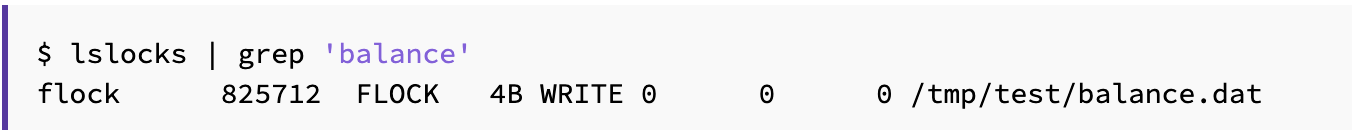
\includegraphics[width=0.8\textwidth]{img/lslocks-balance.png}
    \caption{Capture d'écran de la commande \texttt{lslocks} avec \texttt{balance}}
    \label{fig:lslocks-balance}
\end{figure}
Selon cet output, on peut en déduire que le verrou a été appliqué avec la commande \texttt{flock}, la taille du verrou est de 4B et en mode écriture et qu'il a été appliqué sur le fichier /tmp/test/balance.dat via le process pid=825712
\newline

\textbf{Remarque:} Une démo de ce script est disponible dans l'archive tar que vous pouvez consulter. De plus, le code et les scripts dans entièreté se trouvent sur ce git\cite{git} afin que vous puissiez tester cette expérience dans votre environnement et manipuler les codes à votre guise.
\newline

\subsection{Mandatory Locks}

Jusqu'ici, on pourrait très bien se débrouiller avec des sémahpores. Rien de très révolutionnaire. Mais voyons maintenant l'une des plus grosse différences.
\newline

Les Mandatory locks (verrous obligatoires) sont définis par le noyau et ne peuvent pas être annulés par les processus. La fonction \texttt{fcntl()} est également utilisée pour définir des verrous obligatoires sur les fichiers.

Il ne requiert aucune coopération entre les processus. Si un mandatory locking est activé sur un fichier, c’est l’OS qui prend en charge le verrou et qui avertira les process. Le principe de "celui qui ne joue pas le jeu n'est pas bloqué" n'est donc pas d'actualité.
\newline

Si un processus essaie d'effectuer un accès sur la région d'un fichier qui a un verrou obligatoire, le résultat dépendra de l'attribut \texttt{O\_NONBLOCK} pour son description de fichier. Si l'attribut \texttt{O\_NONBLOCK} n'est pas activé, l'appel système bloquera jusqu'à ce que le verrou soit liberé. Si l'attribut \texttt{O\_NONBLOCK} est activé, l'appel système échouera.
\newline

Dans un environnement où plusieurs utilisateurs accèdent à un fichier, le mandatory locking assure un accès exclusif à un enregistrement. Sans cela, des conflits de mise à jour simultanée pourraient conduire à des pertes de données. Avec le mandatory locking, un utilisateur obtient un verrou exclusif sur l'enregistrement, empêchant d'autres utilisateurs d'y accéder tant que le verrou est détenu. Ce verrou est indépendant des droits du fichier, ni du créateur car le verrou est appliqué directement sur le système de fichier.
\newline

Ils ne sont généralement pas activés par défaut sur les systèmes d'exploitation car il ajoute une complexité supplémentaires aux systèmes de fichiers qui n'en n'ont pas pour la plupart du temps pas besoin.
\newline

Voici les étapes pour activer le mandatory locking sur Linux et leur effet sur le noyau :

\begin{itemize}
  \item Le système de fichiers (FS) doit être monté avec l'option \texttt{mand} :
        \begin{verbatim}
        mount -o mand FILESYSTEM MOUNT_POINT
        \end{verbatim}
    Cela permet d'indiquer au noyau d'activer le support du mandatory locking pour ce système de fichiers particulier. \newline
    
  \item Il faut activer le bit \texttt{set-group-ID} et désactiver le bit \texttt{group-execute} pour tous les fichiers que l'on veut bloquer :
        \begin{verbatim}
        chmod g+s, g-x FILE
        \end{verbatim}
        \texttt{g+s} active le bit set-group-ID sur le fichier. Cela signifie que lorsque le fichier est exécuté, il hérite du groupe du répertoire parent, assurant que tous les membres du groupe ont des droits cohérents.
        \newline
        \texttt{g-x} désactive le bit group-execute sur le fichier, ce qui empêche les membres du groupe d'exécuter le fichier. C'est nécessaire pour ne pas que l'exécution du fichier n'interfére avec le mécanisme de verrouillage.
\end{itemize}

\subsection{L'output de lslocks}
En observant l'output complet de \texttt{lslocks} dans mon terminal, j'ai remarqué qu'il y avait plusieurs locks actifs sur mon système, je me suis donc penché dessus et j'ai observé qu'ils se rapportaient, pour une majorité, à un process en cours d'utilisation. Par exemple, lorsque j'utilise Firefox, le process apporte son lot de verrous. En effet, ils ont tous le même pid et le nom des fichiers verrouillés sont explicites. J'ai fait le test de terminer le process et les locks sont désactivés. Pour mieux comprendre à quoi servent ces verrous j'ai analysé les fichiers sur lesquels ils ont été posés ; les fichiers verrouillés sont en majorité des bases de données locales relatives entre autre aux favoris, aux cookies et d'autres. Les verrous sont de type \texttt{firefox} et qu'ils ont donc leur propre verrou et de type POSIX.

Voici un output concernant les locks de mon systèmes, dont ceux de Mozilla (j'ai volontairement coupé une partie de l'output non-nécessaire pour cette illustration).
\begin{figure}[ht]
  \centering
  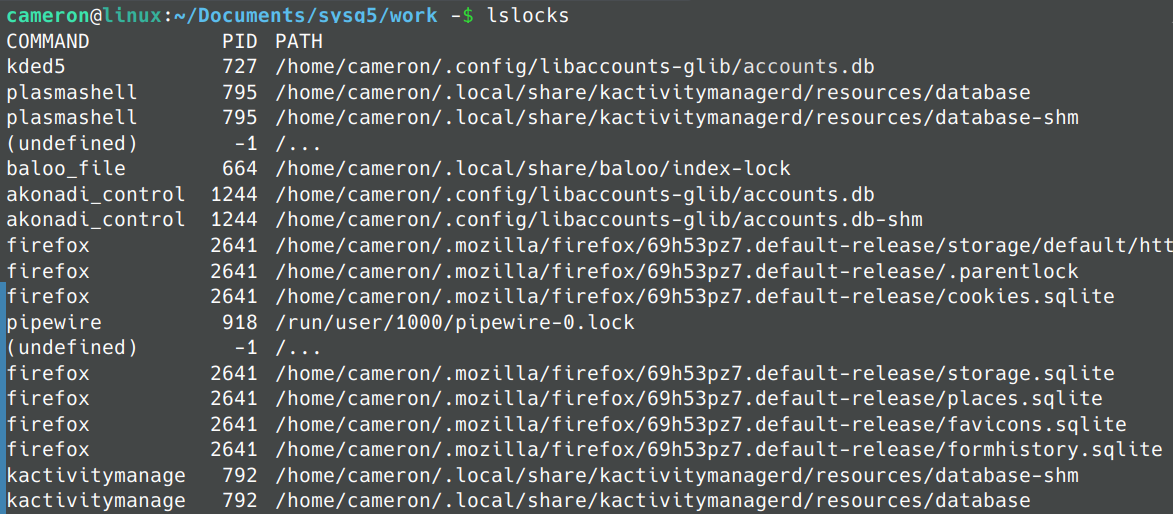
\includegraphics[width=1.0\textwidth, height=8cm]{img/lslock-output.png}
    \caption{Capture d'écran de la commande \texttt{lslocks} avec Mozilla}
    \label{fig:lslocks-mozilla}
\end{figure}
\newline
Je vous invite à faire l'expérience afin de comprendre, sur votre système, quelles sont les potentielles régions critiques.

Pour vous aider à comprendre l'output résultant de la commande, voici les colonnes importantes\cite{ManLslock}
\begin{itemize}
    \item \textbf{COMMAND:} Le nom de la commande ou du processus qui a émis le verrou sur le fichier.
    \item \textbf{PID:} PID du processus qui a émis le verrou.
    \item \textbf{TYPE:} Le type de verrouillage émis sur le fichier (il peut être FLOCK (créé avec flock)  ou  POSIX  (créé  avec fcntl)
    \item \textbf{SIZE:} La taille du verrou en octets.
    \item \textbf{MODE:} Les droits d'accès (lecture, écriture ou * si le process est bloqué).
    \item \textbf{M:} Vaut 1 si verrou obligatoire (mandatory), 0 si requiert coopérativité (1).
    \item \textbf{START:} L'offset à partir duquel le verrou commence dans le fichier.
    \item \textbf{END:} L'offset jusqu'où le verrou s'étend dans le fichier.
    \item \textbf{PATH:} Le chemin complet du fichier verrouillé.
\end{itemize}

Remarque ils n'apparaissent pas tous sur l'image car j'ai réduis les colonnes au minimum. 

    \newpage
\section{La prise en charge par l'OS}

Dorénavant, voyons comment le système d'exploitation s'occupe des verrous.

\subsection{La structure \texttt{flock}}
L'appel système fcntl() se base sur la structure \texttt{flock} pour fonctionnner. Voyons donc comment cette structure se compose et à quoi sert-elle.

\begin{itemize}
    \item \texttt{l\_type} : Il s'agit du type de verrouillage (lecture, écriture, débloquer).
    \newline
    Si le verrouillage est en lecture, un nombre quelconque de processus pourront tenir le verrou (qui sera donc partagé). Un verrou en lecture permet aux processus qui l'acquiert de conserver une cohérence grâce à la synchronisation de l'accès à la ressource. Je ne rentrerai pas plus dans les détails car je n'ai pas plus compris ce point.
    
    Un verrou en écriture se veut quant à lui exclusif. 

    \textbf{Remarque:} 
    Un processus donné ne peut tenir qu'un seul verrou sur une région d'un fichier. Si un nouveau verrou y est appliqué, alors le verrou précédent est converti suivant le nouveau type. Ceci peut entraîner la réduction ou l'extension du verrou existant si le nouveau verrou ne coïncide pas exactement avec celui de l'ancien.
    
    \item \texttt{l\_whence} : Interprétation de \texttt{l\_start} (par exemple, SEEK-SET, etc.).
    
    \item \texttt{l\_start} : Décalage par rapport au début.
    
    \item \texttt{l\_len} : Taille en octets du verrouillage. Si 0, alors verrouiller tous les octets de la position indiquée par \texttt{l\_whence} et \texttt{l\_start} jusqu'à la fin du fichier, quelle que soit sa taille.
\end{itemize}

\subsection{L'appel système fcntl() au niveau de l'OS\cite{ManFnctl}}

\texttt{fcntl} permet d'effectuer plusieurs opérations sur un descripteur de fichier. L'opération à effectuer est déterminée par la valeur de l'argument \texttt{cmd}. \texttt{fcntl} possède 2 ou 3 paramètres selon l'argument \texttt{cmd} : le descripteur de fichier (\texttt{file descriptor}) et la commande (\texttt{cmd}). Le troisième paramètre est adapté en fonction de la commande, dans notre cas, il s'agit d'un pointeur vers la structure \texttt{flock} qui doit posséder au minimum les paramètres donnés dans la section précédente.
    
Dans le cadre du verrouillage de fichiers consultatif (Advisory Lock), le fichier doit être ouvert au sein du process à l'aide d'un file descriptor \texttt{fd}.

Une fois la structure définie, on appelle la fonction \texttt{fcntl} avec le descripteur de fichier (qui doit être ouvert au moins en lecture pour un verrou en lecture et en écriture si le verrou est en écriture) et la commande \texttt{SETLK}. Cela créera soit un verrou en écriture, en lecture, ou le libérera si \texttt{l\_type} vaut \texttt{UNLCK}. En cas de conflit avec un verrou détenu par un autre processus, la fonction renvoie -1 ou bien le process sera bloqué si un de ses flags l'a demandé.

Si un processus qui a créé un verrou est terminé ou s'il ferme un descripteur de fichier d'un fichier sur lequel est appliqué un verrou, alors les verrous créés seront libérés également. Cela a été observé dans mon exemple avec Mozilla Firefox (voir section 4.4).
\newline

\textbf{Remarque:} 
Les verrouillages d'enregistrements ne sont pas hérités par les enfants lors d'un \texttt{fork}, mais sont préservés à travers un \texttt{exec}.

Lorsqu'un processus utilise la fonction \texttt{fork}, il crée une copie du processus parent, appelée processus fils. Cette copie inclut les descripteurs de fichiers ouverts, y compris les verrous associés à ces descripteurs de fichiers. Il est important de noter que cela ne crée pas une copie physique des verrous; au lieu de cela, les deux processus (le parent et le fils) partagent les mêmes verrous.

Si le processus fils ou le processus parent modifie l'état du verrou, cette modification sera reflétée dans l'autre processus, car ils partagent le même espace de descripteurs de fichiers.

Cependant, lorsqu'un processus utilise \texttt{execve} pour exécuter un nouveau programme, le système d'exploitation remplace l'image du processus en cours par celle du nouveau programme. 


    \newpage
\section{L'implémentation des verrous}

\subsection{Gestion d'une région critique grâce à un verrouillage}
Je vais à présent démontrer comment protéger une région critique avec les verrouillages en language C grâce à la structure \texttt{flock} et l'appel système \texttt{fcntl}. Nous étudierons plus en profondeur cet AS dans la suite de ce rapport.
\newline
Dans l'exemple qui suit, nous allons essayer de sécuriser l'accès à une base de données locale afin de conserver une cohérence à tout moment.

\begin{mdframed}[style=mystyle]
\begin{lstlisting}[language=C, caption={Code C avec verrouillage de fichier}]
#include <stdio.h>
#include <stdlib.h>
#include <string.h>
#include <unistd.h>
#include <fcntl.h>
#include <sys/wait.h>

int main(int argc, char *argv[]) {
    int fd, n;
    char buff[100];

    // Ouverture du fichier de la base de donnees
    if ((fd = open("database.txt", O_WRONLY | O_CREAT 
            | O_TRUNC, 0666)) == -1) {
        perror("open");
        exit(-1);
    }

    // Configuration du verrou via la structure flock
    struct flock lock;
    lock.l_type = F_WRLCK;  // Verrou en ecriture
    lock.l_whence = SEEK_SET;
    lock.l_start = 0;
    lock.l_len = 0;  // Verrou sur tout le fichier

    if (fcntl(fd, F_SETLKW, &lock) == -1) {
        perror("fcntl");
        exit(1);
    }

    if (fork() == 0) {
        // Code du fils
        while (fcntl(fd, F_GETLK, &lock) != -1 
                && lock.l_type != F_UNLCK) {
            sleep(1);
        }

        do {
            printf("[fils]: a pris le verrou sur la database\n");
            n = read(0, buff, 100);
            buff[n - 1] = 0;
            printf("[fils]: rend le verrou\n");

            if (fcntl(fd, F_SETLKW, &lock) == -1) {
                perror("[fils] fcntl");
                exit(1);
            }

            write(fd, buff, n);

            if (fcntl(fd, F_SETLK, &lock) == -1) {
                perror("[fils] fcntl");
                exit(1);
            }
        } while (strcmp(buff, "quit") != 0);

        printf("[fils]: a termine\n");
        exit(0);
    }
    else {
        // Code du pere
        while (fcntl(fd, F_GETLK, &lock) != -1 
                && lock.l_type != F_UNLCK) {
            sleep(1);
        }

        do {
            printf("[pere]: a pris le verrou sur la database\n");
            n = read(0, buff, 100);
            buff[n - 1] = 0;
            printf("[pere]: rend le verrou\n");


            if (fcntl(fd, F_SETLKW, &lock) == -1) {
                perror("[pere] fcntl");
                exit(1);
            }

            write(fd, buff, n);

            if (fcntl(fd, F_SETLK, &lock) == -1) {
                perror("[pere] fcntl");
                exit(1);
            }
        } while (strcmp(buff, "quit") != 0);

        printf("[pere]: a termine\n");
        wait(0);
    }

    // Fermeture du fichier (le verrou sera libere)
    close(fd);
    exit(0);
}
\end{lstlisting}
\end{mdframed}
\paragraph{Explication :}
Dans ce code, nous utilisons la fonction `fcntl` pour établir un verrou obligatoire sur le fichier "database.txt". Le verrou  est configuré en écriture et couvre l'ensemble du fichier. 

Lorsqu'un processus tente d'accéder au fichier qui a un verrou obligatoire, le système d'exploitation vérifie si le verrou est déjà détenu par un autre processus. Si le verrou est disponible, le processus qui a tenté d'acquérir le verrou réussira et pourra accéder au fichier. En revanche, si le verrou est déjà détenu par un autre processus, le système d'exploitation bloquera le processus en attente jusqu'à ce que le verrou soit libéré par le processus actuel propriétaire du verrou.

Cela garantit qu'un seul processus à la fois peut détenir le verrou obligatoire sur le fichier, assurant ainsi un accès exclusif à la ressource. Les autres processus qui tentent d'acquérir le verrou pendant qu'il est déjà détenu par un processus doivent attendre que le verrou soit libéré.

\paragraph{Remarque :} Notez qu'il s'agit la d'une implémentation d'un verrou consultatif (Adivsory Lock) et qu'il requiert donc coopérativité. Malheureusement, monter le système de fichiers pour qu'il soit compatibles avec les verrous obligatoires (Mandatory Lock) demande d'avoir les droits d'administrateurs, ce qui n'est pas possible au local 503. Cependant, leur implémentation est très similaire après avoir monter le système de fichier comme décrit à la section 4.3. Cela implique que dans mon exemple et ma démo, les 2 processus se doivent d'être coopératifs.

\subsection{Comparaison avec un sémaphore}
Nous venons donc de voir comment verrouiller un ficher avec des locks, je décide donc à présent d'illustrer la comparaison avec un sémaphore qui ferait la même action. Analysons la mise en place de gestion d'une région critique sur une base de données locale avec un sémaphore

\begin{mdframed}[style=mystyle]
\begin{lstlisting}[language=C, caption={Code C avec sémaphore}]
#include <sys/types.h>
#include <sys/ipc.h>
#include <sys/sem.h>
#include <stdio.h>
#include <stdlib.h>
#include <string.h>
#include <unistd.h>

#define SEM_KEY 1234

int opsem(int sem, int i) {
    struct sembuf op[1];
    op[0].sem_num = 0;
    op[0].sem_op = i;
    op[0].sem_flg = 0;

    if (semop(sem, op, 1) == -1) {
        perror("semop");
        exit(1);
    }
    return 0;
}

int main(int argc, char *argv[]) {
    int sem, n;
    char buff[100];

    // Creation du semaphore
    if ((sem = semget(SEM_KEY, 1, 0666 | IPC_CREAT)) == -1) {
        perror("semget");
        exit(-1);
    }

    // Initialisation du semaphore
    if (semctl(sem, 0, SETVAL, 1) == -1) {
        perror("semctl");
        exit(1);
    }

    if (fork() == 0) {
        do {
            opsem(sem, -1); // down
            printf("[fils]: I want access to the database\n");
            n = read(0, buff, 100);
            buff[n - 1] = 0;
            printf("[fils]: Wrote: [%s]\n", buff);
            opsem(sem, +1); // up
        } while (strcmp(buff, "quit") != 0);
        printf("[fils]: Access to the database done\n");
        exit(0);
    }

    do {
        opsem(sem, -1); // down
        printf("[pere]: I want access to the database\n");
        n = read(0, buff, 100);
        buff[n - 1] = 0;
        printf("Wrote: [%s]\n", buff);
        opsem(sem, +1); // up
    } while (strcmp(buff, "quit") != 0);

    printf("[pere]: Access to the database done\n");
    wait(0);

    // Suppression du semaphore
    if (semctl(sem, 0, IPC_RMID) != 0) {
        perror("semctl");
        exit(1);
    }
    exit(0);
}
\end{lstlisting}
\end{mdframed}

\paragraph{Explication :}
Sans rentrer dans les détails de l'implémentation des sémaphores étant donné que l'on a déjà étudier ce concept précédemment, on obsèrve dans un premier temps que pour un même but, le sémaphore demande bien plus de code et de mise en place. Chaque process voulant opérer une région critique doit se rappeler qu'il doit faire appel au sémaphore, potentiellement devoir l'initialiser

\subsection{Les différences entre ces 2 manières}
\textbf{Avantages des locks :}

\begin{itemize}
\item \textit{Simplicité d'implémentation :} Le code avec les verrous de fichier est souvent plus concis et plus facile à comprendre. L'utilisation de la structure \texttt{flock} et de \texttt{fcntl} simplifie la gestion des verrous, offrant une abstraction plus conviviale.

\item \textit{Intégration avec le système de fichiers :} Les verrous de fichier s'intègrent naturellement avec le système de fichiers, offrant une approche transparente pour contrôler l'accès aux ressources partagées.
\end{itemize}

\textbf{Nuances et Considérations :}

\begin{itemize}
\item \textit{Complexité de la Sémantique des Verrous :} Bien que les verrous de fichier soient simples à mettre en œuvre, la sémantique des verrous peut parfois être complexe. Par exemple, un verrou en écriture peut bloquer d'autres verrous en lecture, ce qui peut entraîner des comportements inattendus dans certaines situations. En effet, un verrou en lecture peut être partagé contrairement à un verrou en écriture. Si un nouveau verrou est appliqué sur une zone déjà verrouillée, alors le verrou précédent est converti suivant le nouveau type. Cette conversion peut alors réduire ou étendre le verrou existant et corrompre l'accès.
\item \textit{Flexibilité des Sémaphores :} Les sémaphores offrent une plus grande flexibilité dans la gestion de l'accès concurrent. Ils permettent de définir des politiques plus complexes, comme la priorité entre différents processus ou la gestion fine des autorisations d'accès.
\end{itemize}

En conclusion, bien que les verrous de fichier soient une option attractive en raison de leur simplicité et de leur portabilité, les sémaphores peuvent être préférables dans des cas où une flexibilité accrue et une gestion fine de l'accès sont nécessaires. Le choix entre les deux dépendra des exigences spécifiques de l'application et des performances souhaitées.
    \newpage
\section{Conclusion}
Ce rapport m'a permis d'atteindre les objectifs fixés, à savoir comprendre le fonctionnement des verrouillages de fichiers, utiliser ces outils, et explorer les concepts de manière autonome.

À travers cette exploration, j'ai pu découvrir le rôle des verrous dans la gestion de l'accès concurrentiel aux fichiers et l'importance de ces mécanismes pour assurer une exécution sécurisée et cohérente des opérations dans un environnement multi-processus.

Le récapitulatif des types de verrouillages, qu'ils soient advisory ou mandatory, ainsi que la prise en charge par le système d'exploitation à travers les structures \texttt{flock} et les appels système \texttt{fcntl()}, ont contribué à enrichir mes connaissances sur la manière dont le noyau gère ces opérations.

J'ai également réalisé l'importance de considérer le comportement de ces mécanismes lors de la création de processus fils, notamment dans le contexte de l'utilisation de \texttt{fork} et \texttt{execve}. Cela m'a fait comprendre qu'un fork n'est pas sans risque et qu'il y a une multitude de chose à faire lorsque l'on clone un process pour en faire un fils étant donné qu'ils partagent les mêmes descripteurs de fichiers, ...

En somme, ce travail a été une opportunité de découvrir un nouvel outil en programmation système, tout en suscitant une réflexion approfondie sur la nécessité de garantir une concurrence cohérente dans la gestion des ressources partagées.
\newpage

% ------------------------------------------------------------------------------
% Reference and Cited Works
% ------------------------------------------------------------------------------

\bibliographystyle{plain}
\bibliography{references.bib}

% ------------------------------------------------------------------------------

\end{document}
